\section{System Exploration and Findings}

This section summarizes the exploration process, focusing on understanding the structure, tables, and solutions used in the NBS system.

\subsection{Overview}

To understand the current state of the system, its structure, components, and data were thoroughly explored. This section presents the findings from this exploration, focusing on the tables, solutions, and Power BI reports that form the core of the NBS system.

The exploration began with an analysis of tables within NBS. They were examined to understand their structure, the relationships between them, and the quality of the data they contain. Additionally, the system's solutions were reviewed and listed.

Furthermore, the exploration included a review of the Power BI reports used to visualize the data. Along with tables and solutions, these reports were also comprehensively inventorized.

This section includes a detailed inventory of the tables, solutions, and reports. These findings serve as the foundation for the subsequent analysis, providing a clear picture of the NBS components.

\subsection{Tables}

The tables in the NBS system are referred to as "entities." In the Microsoft Dataverse structure, each entity has a logical name (its technical identifier) and a display name, which is more user-friendly and shown in the application's frontend.

While exploring the system, it appeared that tables related to NBS often start with one of the following prefixes: \texttt{cr675\_}, \texttt{cr91b\_}, or \texttt{craab\_}. As the Microsoft Dataverse API returns a list of all tables, these prefixes served as flags when identifying which tables could be related to NBS. This approach narrowed down the search from hundreds of tables to several dozen.

Another indication of which tables were in use was the \texttt{Data Analyzer} Power BI report.

\newpage

\subsubsection{List of Tables}

This is a list of tables used by NBS. The end user typically recognizes tables by their display names, while the logical names are used for programmatic interactions with the system.

\begin{footnotesize}
	\begin{tabularx}{\textwidth}{l|l}
		\textbf{Display Name} & \textbf{Logical Name} \\\hline\\
		\textbf{NBS Test Action} & \texttt{cr675\_testdashboardtestprocedment} \\[0.5em]
		\textbf{IFS MATERIALS V3} & \texttt{cr675\_ifsmaterialsv3} \\[0.5em]
		\textbf{NBS Construction Material Stacks Stitchings} & \texttt{cr675\_nbsconstructionmaterialstacksstitchings} \\[0.5em]
		\textbf{NBS IFS MATERIALS} & \texttt{cr675\_nbsifsmaterials} \\[0.5em]
		\textbf{NBS Material stack} & \texttt{cr675\_nbsmaterialstack} \\[0.5em]
		\textbf{NBS Sample} & \texttt{cr675\_testdashboardsample} \\[0.5em]
		\textbf{NBS Test Compound} & \texttt{cr675\_testcompounds} \\[0.5em]
		\textbf{NBS Test Order} & \texttt{cr675\_testorder} \\[0.5em]
		\textbf{NBS ICW Products} & \texttt{cr675\_nbsicwproducts} \\[0.5em]
		\textbf{NBS R Table} & \texttt{cr91b\_nbsrtable} \\[0.5em]
		\textbf{NBS Ballistic System} & \texttt{cr675\_testdashboardballisticsystem} \\[0.5em]
		\textbf{NBS Construction} & \texttt{cr675\_nbsconstruction} \\[0.5em]
		\textbf{NBS Product} & \texttt{cr675\_testdashboardproduct} \\[0.5em]
		\textbf{NBS FREC2 RND Orders} & \texttt{cr675\_nbsfrec2rndorders} \\[0.5em]
		\textbf{NBS Operation} & \texttt{cr675\_nbsstitching} \\[0.5em]
		\textbf{NBS Material} & \texttt{cr675\_nbsmaterial} \\[0.5em]
		\textbf{NBS Test Protocol Template} & \texttt{cr675\_testdashboardstandarddetails} \\[0.5em]
		\textbf{NBS Bullet Type Dictionary} & \texttt{cr675\_testdashboardammotypedictionary} \\[0.5em]
		\textbf{NBS Project} & \texttt{cr675\_project} \\[0.5em]
		\textbf{NBS Geometry} & \texttt{cr675\_testdashboardgeometries} \\[0.5em]
		\textbf{NBS Group Order} & \texttt{craab\_nbsgrouporder} \\[0.5em]
		\textbf{NBS MaterialStackAndConstraction} & \texttt{cr675\_nbsmaterialstackandconstraction} \\[0.5em]
		\textbf{NBS Program} & \texttt{cr91b\_nbsprogram} \\[0.5em]
		\textbf{NBS Standard Names Dictionary} & \texttt{cr675\_testdashboardstandard} \\[0.5em]
		\textbf{NBS Preliminary Testing} & \texttt{cr675\_nbspreliminarytesting} \\[0.5em]
		\textbf{NBS Backing Type Dictionary} & \texttt{cr675\_nbstestdashboardbackingtypedictionary} \\[0.5em]
		\textbf{NBS Cartridge Type Dictionary} & \texttt{cr675\_nbstestdashboardcartridgetypedictionary} \\[0.5em]
		\textbf{NBS Institute} & \texttt{cr675\_testdashboardinstitute} \\[0.5em]
		\textbf{R\&DOrderView} & \texttt{cr675\_orderviewrd} \\[0.5em]
		\textbf{NBS FRECII Tool Type} & \texttt{craab\_nbstooltype} \\[0.5em]
		\textbf{NBS Powder Type Dictionary} & \texttt{cr675\_nbstestdashboardpowdertypedictionary} \\[0.5em]
		\textbf{NBS Photo} & \texttt{cr675\_testdashboardphotos} \\[0.5em]
	\end{tabularx}
\end{footnotesize}

\subsubsection{Entity Relationship Diagram}

This is the Entity Relationship Diagram (ERD) of the main tables used in NBS. It provides an overview of the relationships between tables and offers suggestions for potential table merging during data preparation.

\begin{figure}[h!]
\centering
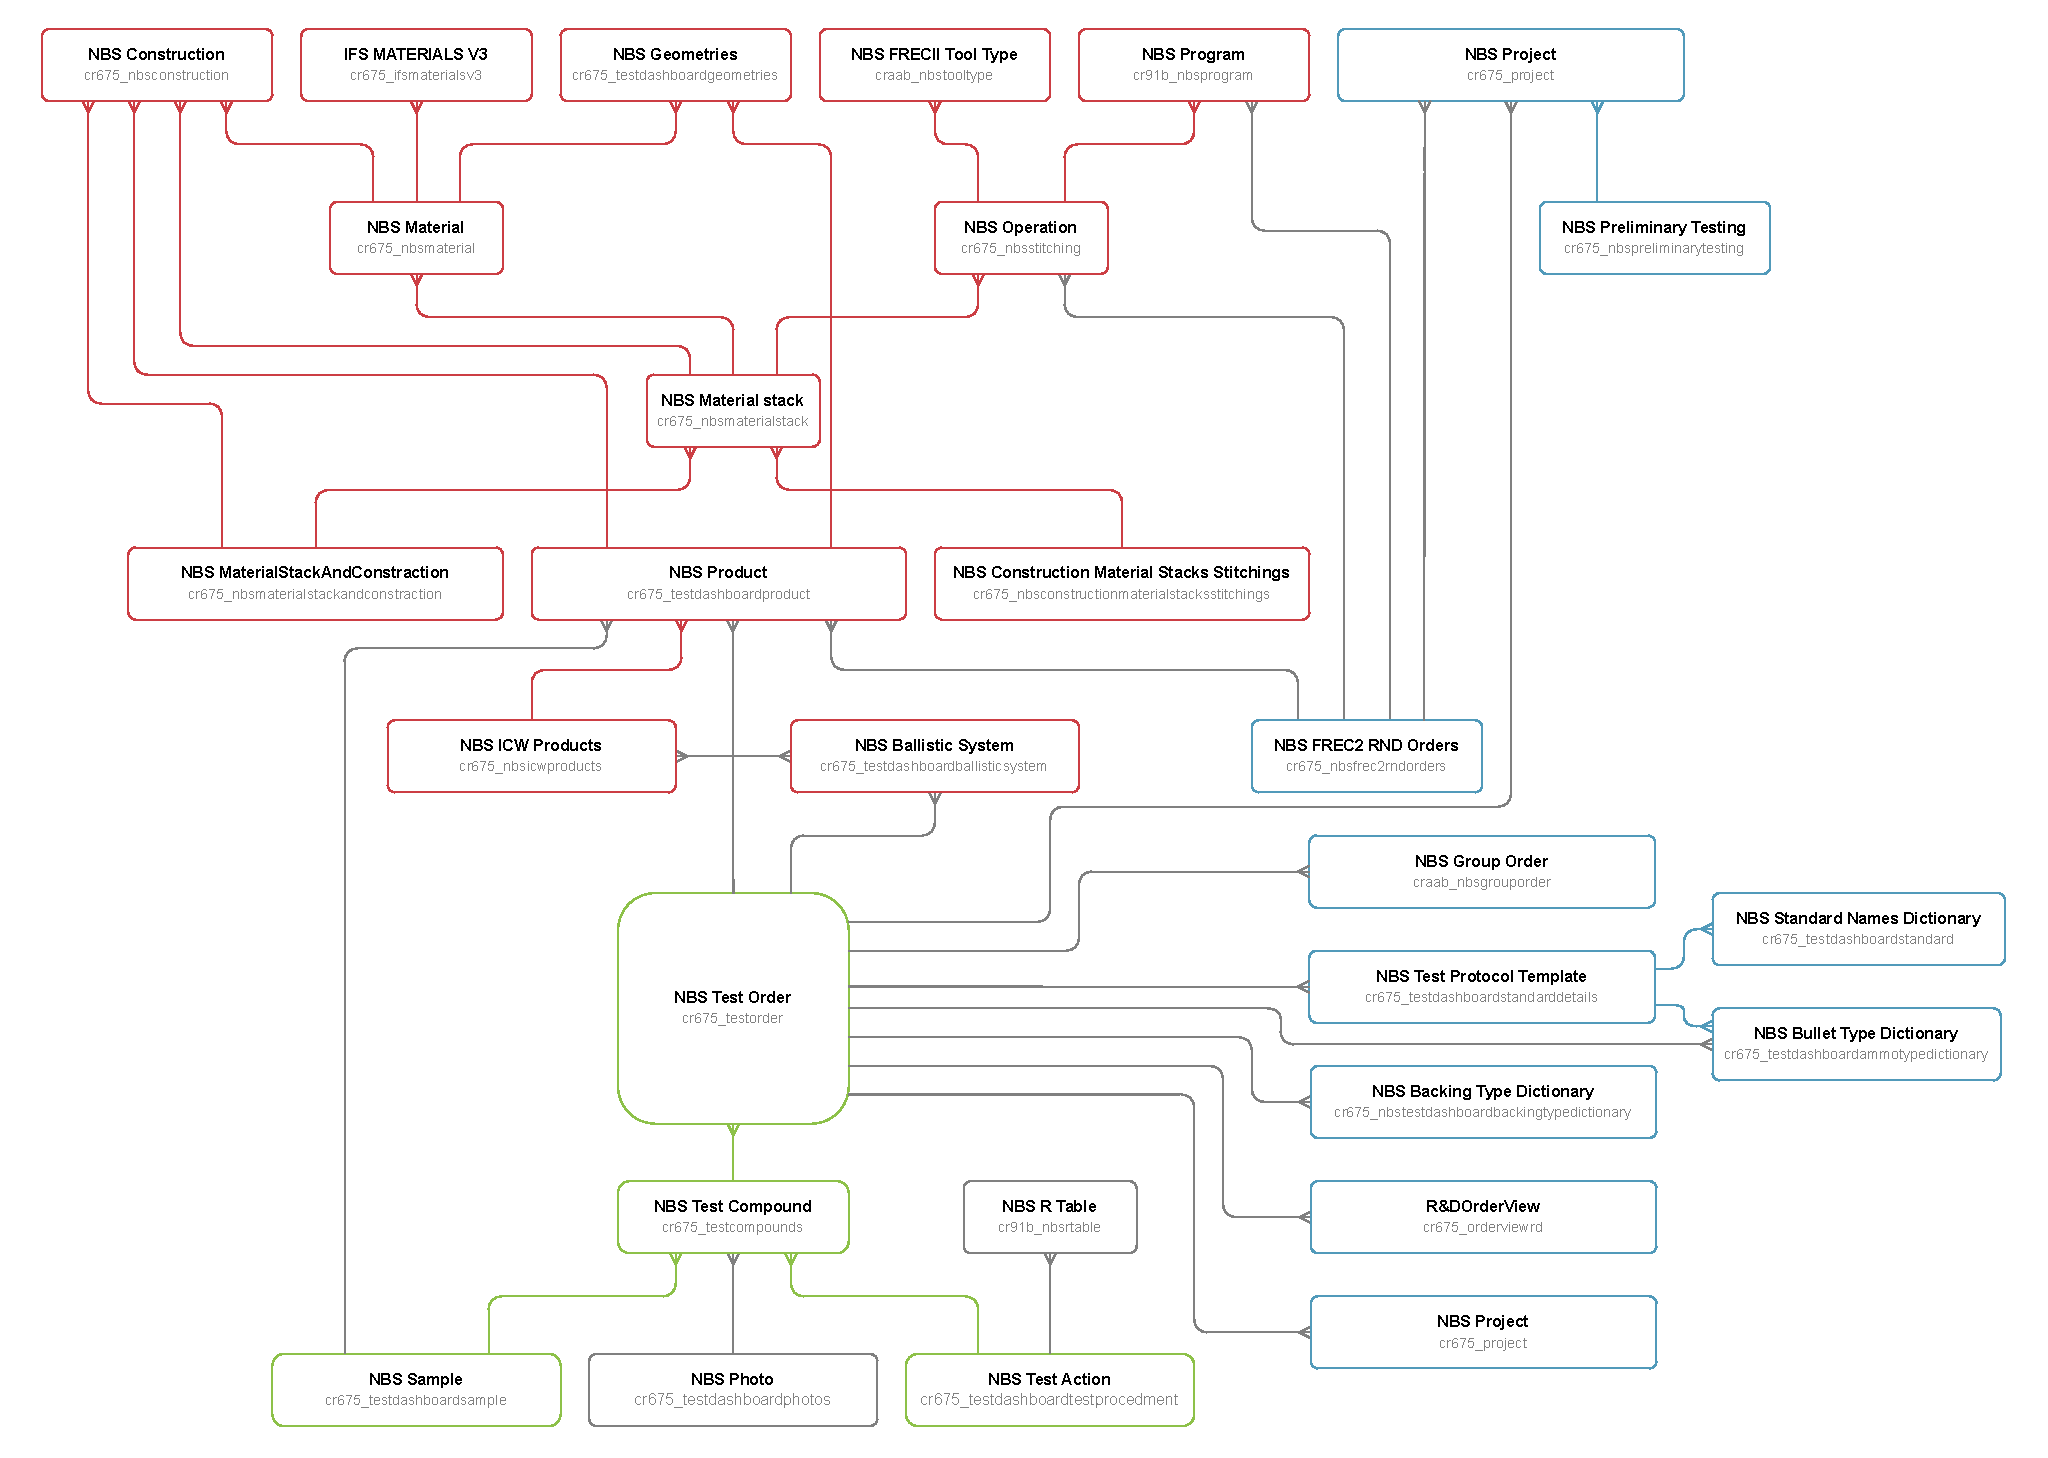
\includegraphics[width=\textwidth]{PDFs/er_diagram.pdf}
\end{figure}

The diagram uses Barker's Notation for entity relationships. For reference see \href{https://ece.uprm.edu/~icom5047/documents/barkers-erd-notation.pdf}{Barker's ERD Notation}

Colors used in the diagram are used for logical grouping of tables:
\begin{itemize}
    \item Tables related to \textcolor[HTML]{cc3e44}{materials/constructions} are highlighted in \textcolor[HTML]{cc3e44}{red}.
    \item Tables related to \textcolor[HTML]{8dc149}{tests} are highlighted in \textcolor[HTML]{8dc149}{green}.
    \item Tables which serve as \textcolor[HTML]{519aba}{dictionaries/indexes} are highlighted in \textcolor[HTML]{519aba}{blue} (these are the first ones to be merged when doing data preparation).
    \item Tables which are \textcolor[HTML]{808080}{useless/obsolete} are highlighted in \textcolor[HTML]{808080}{gray}.
\end{itemize}



\subsubsection{Detailed Inventory of Tables}

This section contains a detailed inventory of tables, including row and column counts, table relationships, and a list of columns. The full inventory is available in the \hyperref[sec:Appendices]{Appendices} section in multiple formats (.json, .pdf, and .md).

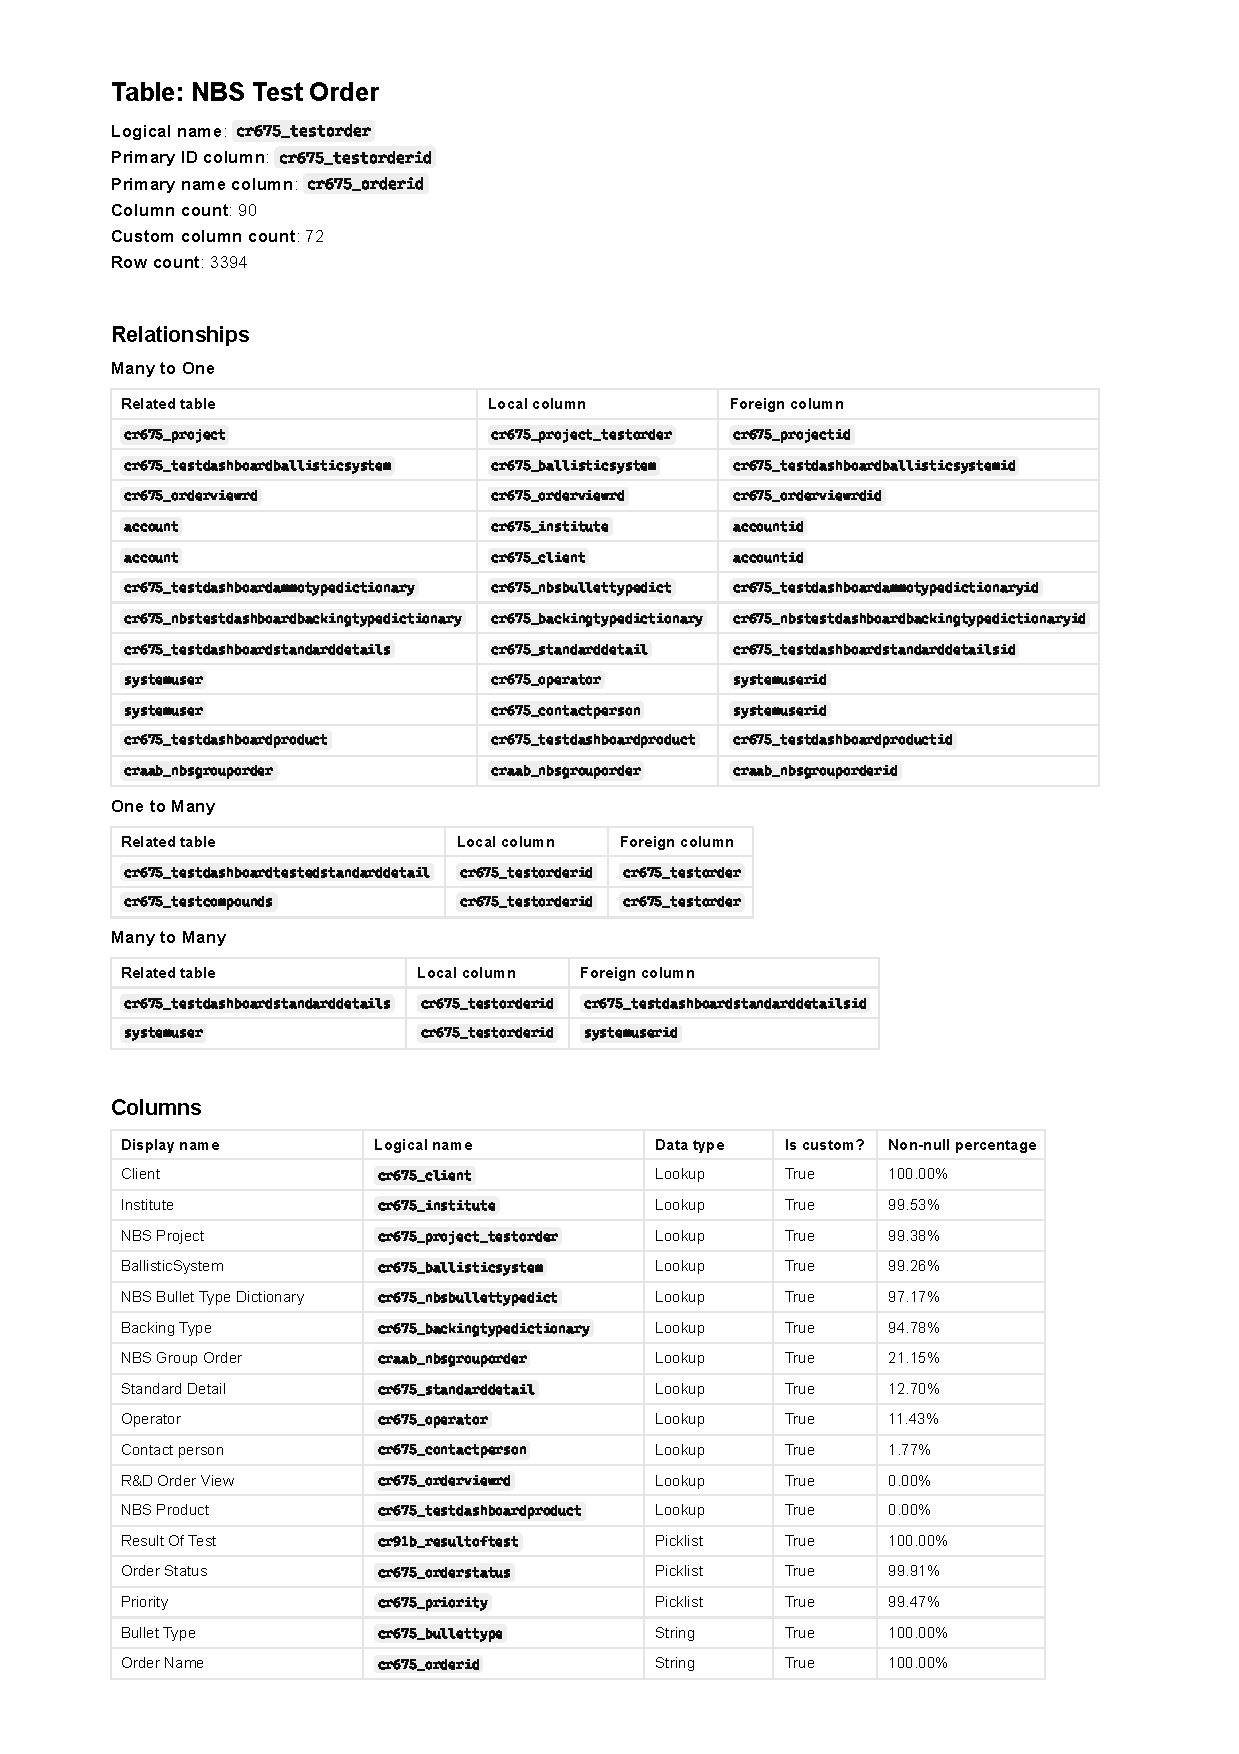
\includepdf[pages=-]{PDFs/tables_markdown.pdf}

\subsection{Solutions}

A \textbf{solution} is a logical container for components such as tables, apps, dashboards, and other resources related to a specific process or system. Solutions are crucial for organizing and managing system components, especially when moving them between environments.

As described by Microsoft:

\begin{quote}
	\textit{Solutions are used to transport apps and components from one environment to another or to apply a set of customizations to existing apps. A solution can contain one or more apps as well as other components such as site maps, tables, processes, web resources, choices, flows, and more.} \\
	\href{https://learn.microsoft.com/en-us/power-apps/maker/data-platform/solutions-overview}{Source}
\end{quote}

In the context of the NBS system, identifying associated solutions is essential for migrating the system from the current NFM Group Def environment to the NFM Group NBS DEV environment. Proper identification and organization of these solutions will ensure seamless migration of all related components, including tables, apps, and workflows.

Each solution has a \textbf{display name} for easy identification and a \textbf{unique name}, which serves as a system-level identifier. This distinction is crucial for managing solutions during customization and migration processes.

\subsubsection{List of Solutions Related to NBS}

\begin{small}
	\begin{tabularx}{\textwidth}{l|l}
		\textbf{Display name} & \textbf{Unique name} \\
		\hline
		Ribbon\_1 & \texttt{Ribbon\_1} \\
		Ribbon\_2 & \texttt{Ribbon\_2} \\
		Ribbon\_3 & \texttt{Ribbon\_3} \\
		Ribbon\_4 & \texttt{Ribbon\_4} \\
		Ribbon\_5 & \texttt{Ribbon\_5} \\
		NBS Product & \texttt{NBSProduct} \\
		NBS Construction & \texttt{NBSConstruction} \\
		Balistic System & \texttt{BalisticSystem} \\
		NBS Geometry & \texttt{NBSGeometry} \\
		NBSTestOrder & \texttt{NBSTestOrder} \\
		NBS Project & \texttt{NBSProject} \\
		NBS PreliminaryTest & \texttt{PreliminaryTest} \\
		Backing Type & \texttt{BackingType} \\
		NBS Model-Driven & \texttt{NBSModelDriven} \\
		NBS Apps & \texttt{NBSApps} \\
		remove dependencies & \texttt{removedependencies} \\
		NBS Migration & \texttt{NBSMigration} \\
		NBS Tester & \texttt{NBSTester} \\
		Construction Creator Model Driven & \texttt{ConstructionCreatorModelDriven} \\
		NBS Database & \texttt{NBSDatabase} \\
		NBS Data Base for migration & \texttt{NBSDataBaseformigration} \\
		NFM BallisticDB & \texttt{NFMBallisticDB} \\
		Account & \texttt{Account} \\
		Common Data Services Default Solution & \texttt{Crb118a} \\
	\end{tabularx}
\end{small}

\subsubsection{Inventory of Solutions Related to NBS}

Below is a comprehensive inventarization of solutions along with their components such as tables and apps.

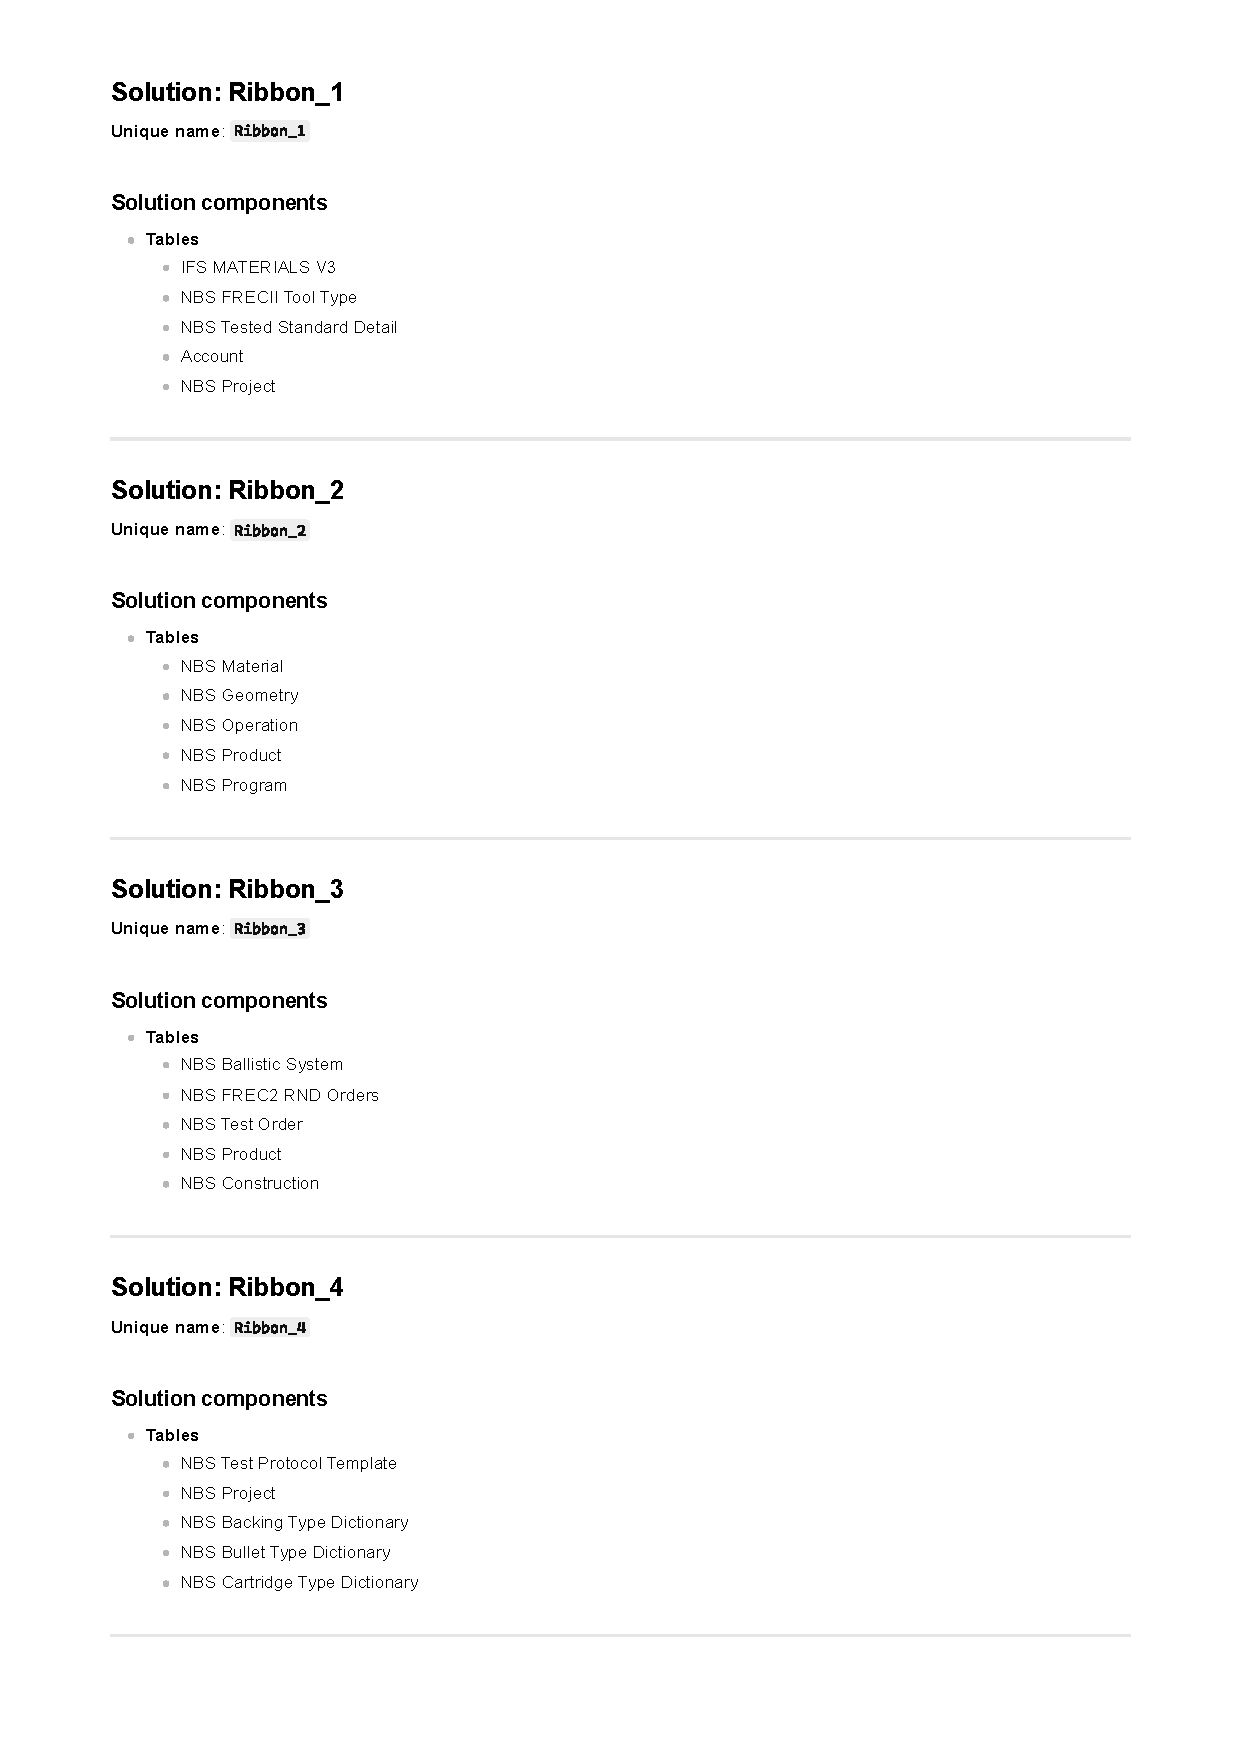
\includepdf[pages=-]{PDFs/solutions_markdown.pdf}

\subsection{Reports}

A key task in this project was to conduct a detailed review of all Power BI reports used in the NBS Workspace.

\subsubsection{List of Reports Related to NBS}

\begin{small}
	\begin{tabularx}{\textwidth}{l|l}
		\textbf{Report name} & \textbf{Semantic model used} \\
		\hline
		Count of Tested Samples & \texttt{Count of Tested Samples} \\
		Pressed plates count & \texttt{Pressed plates count} \\
		NBS Report Test Range Monitor PL & \texttt{NBS Report\_Test Range Monitor} \\
		NBS Report\_Test Range Monitor & \texttt{NBS Report\_Test Range Monitor} \\
		NBS Report & \texttt{NBS Report} \\
		NBS BSR v1 & \texttt{NBS Report} \\
		NBS Report\_Eabs analysis & \texttt{NBS Report} \\
		NBS Report\_Eabs analysis\_Terje\_cleaned2 & \texttt{NBS Report} \\
	\end{tabularx}
\end{small}

\subsubsection{Inventory of Reports Related to NBS}

Below is a comprehensive inventory of all reports in the NBS Workspace. Each report includes a description, a list of available pages, filters, graphs, and the tables it utilizes.

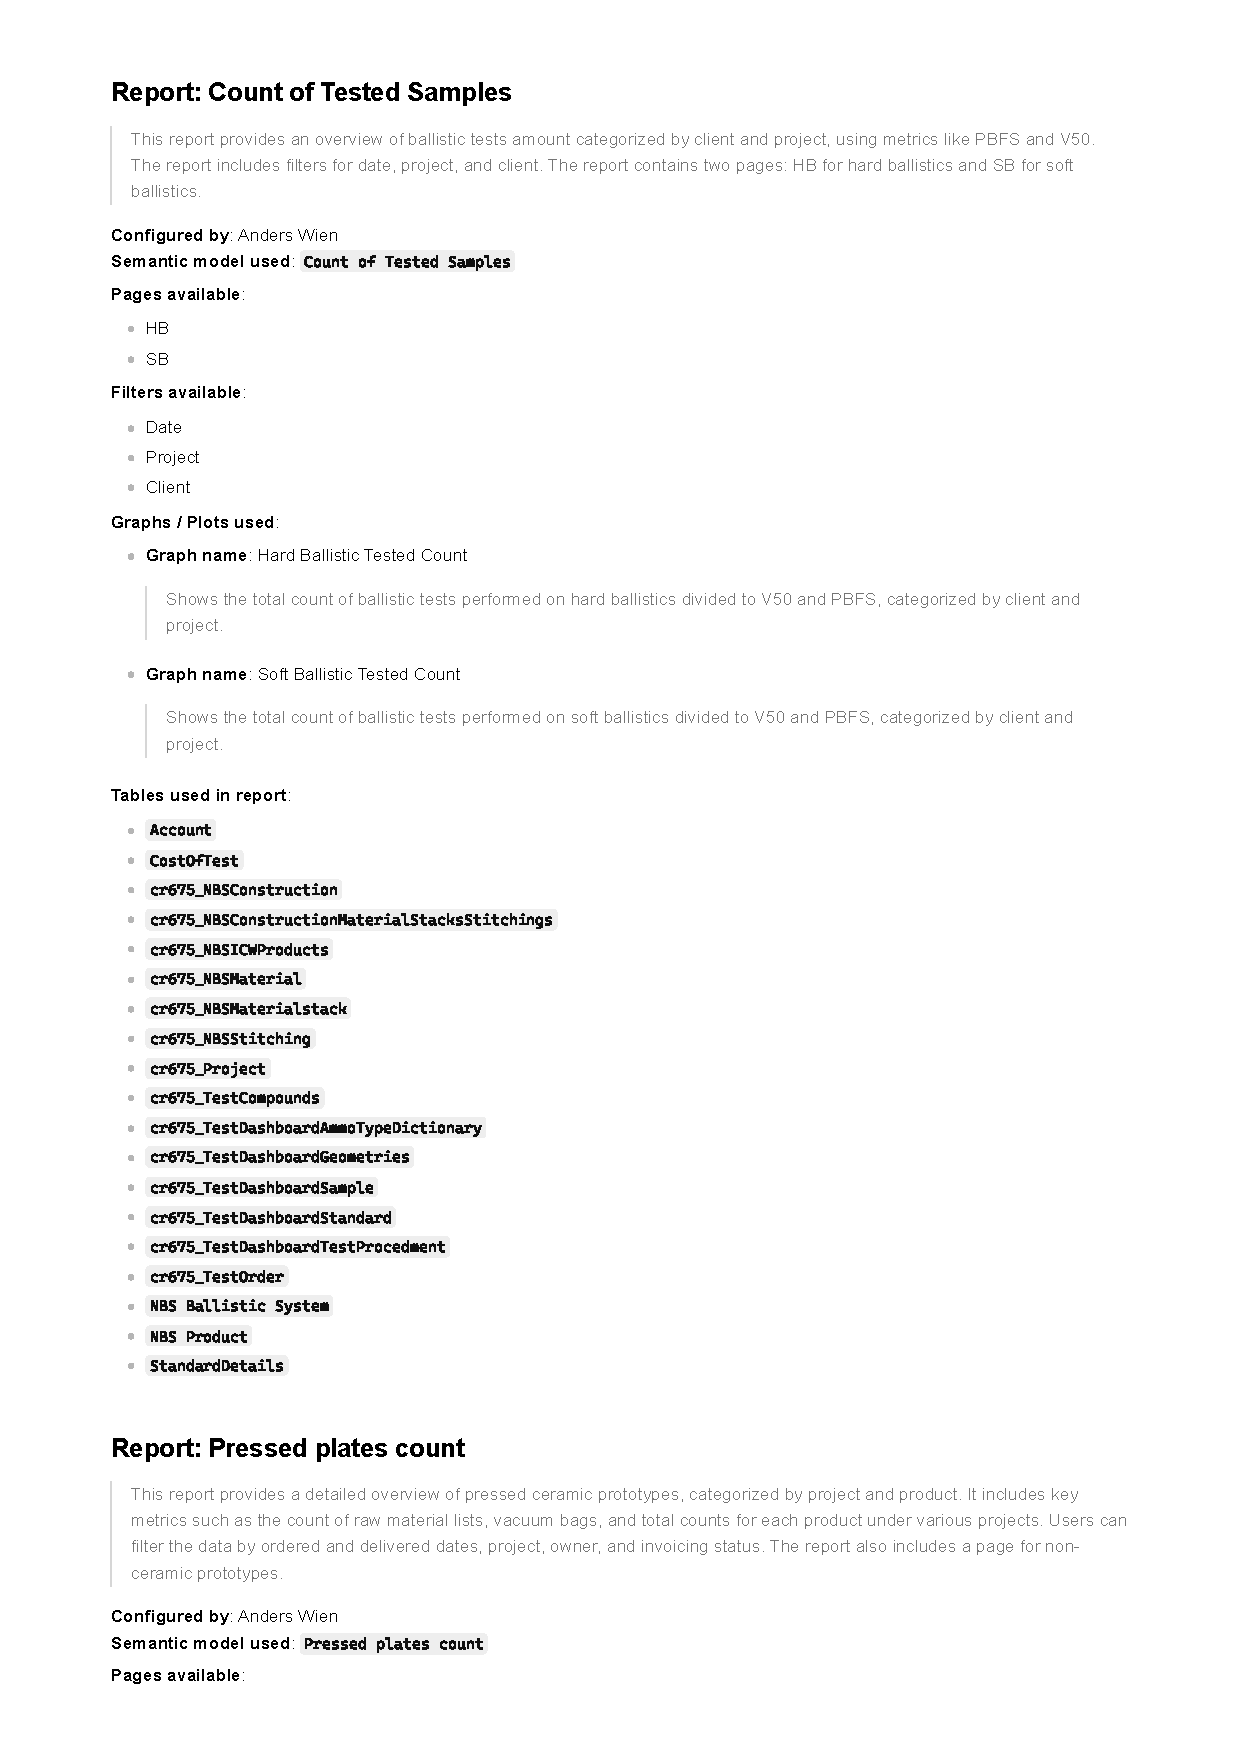
\includepdf[pages=-]{PDFs/reports_markdown.pdf}